\documentclass{beamer}
\usetheme{Warsaw}
%\usecolortheme{seahorse}
\usepackage{graphicx}
\usepackage[utf8]{inputenc}
\usepackage[T1]{fontenc}
\title{C++0x performance improvements}
\author{Łukasz Milewski}
\institute{Uniwersytet Wrocławski}
\date{\today, Wrocław}

\begin{document}

\begin{frame}
  \titlepage
\end{frame}

\begin{frame}
  \tableofcontents
\end{frame}

\begin{frame}{g++}
  \begin{block}{version}
    \$ g++ --version
    g++ (GCC) 4.5.2
  \end{block}
\end{frame}

\section{move semantics and perfect forwarding}
\begin{frame}{rationale}
  \begin{block}{Why?}
    \begin{itemize}
    \item Eliminate expensive copying
    \item Solve problems with generic forwarding
    \item Solve usability problems where binding a rvalue to non-const reference is not a logical error
    \end{itemize}
  \end{block}
\end{frame}

\subsection{lvalue, rvalue and rvalue reference}
\begin{frame}{expression category taxonomy}
  \begin{center}
    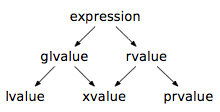
\includegraphics[5cm]{valuetaxonomy.png}
  \end{center}
\end{frame}

\begin{frame}{lvalue, rvalue, rvalue reference}
  \begin{block}{lvalue}
    \begin{itemize}
    \item Can appear on left-hand side of an assignment expression
    \item if E is expr of pointer type, then *E is an lvalue
    \item calling function whose return type is an lvalue reference is lvalue
    \end{itemize}
  \end{block}

  \begin{block}{rvalue}
    \begin{itemize}
    \item can appear on right-hand side of an assignment expression
    \item xvalue
    \item temporary object
    \item value that is not assosiated with an object
    \end{itemize}
  \end{block}
\end{frame}

\begin{frame}{example}
  see rvalue\_lvalue.cpp
\end{frame}

\begin{frame}
  \begin{block}{rvalue reference}
    \begin{itemize}
    \item T\& - lvalue reference
    \item T\&\& - rvalue reference
    \item const T\&\&
    \item binds to lvalues and rvalues
    \item binds to rvalue even if not const qualified
    \end{itemize}
  \end{block}
\end{frame}

\begin{frame}{binding}
  \begin{block}{binding}
  \item lvalue ref binds to lvalue
  \item const lvalue ref binds to everything
  \item rvalue ref binds to lvalue and nonconst rvalue
  \item const rvalue ref binds to everything
  \end{block}
  see binding.cpp
\end{frame}

\begin{frame}{overload resolution}
  see rvalue\_ref\_resolution.cpp
\end{frame}

\subsection{usability improvements}
\begin{frame}{forwarding arguments}
  \begin{block}{binder problem}
    \begin{itemize}
    \item let's write std::binder2nd class
    \item unbound paramters should behave identically to the corresponding parameters in the original function
    \item const lvalue ref should bind to both lvalue and rvalue
    \item non-const lvalue ref should bind to a non-const lvalue
    \item non-const lvalue should refuse to bind to rvalues and const lvalues
    \end{itemize}
  \end{block}
\end{frame}

\begin{frame}{forwarding arguments in C++03}
\begin{verbatim}
template <class Operation>
class binder2nd
    : public unary_function<...>
{
    ...
public:
    ...
    result_type operator()(const first_argument_type\& x);
    result_type operator()(      first_argument_type\& x);
};

\end{verbatim}
\begin{block}{}
  Unfortunately number of overloads grows exponentially with number of
  parameters
\end{block}
\end{frame}

\begin{frame}{forwarding arguments in C++0x}
  \begin{block}{}
\begin{verbatim}
template <class Operation>
class binder2nd
    : public unary_function<...>
{
    ...
public:
    ...
    result_type operator()(first_argument_type\&\& x);
};

\end{verbatim}
  \end{block}
\end{frame}

\begin{frame}{move semantics}
\begin{block}{}
\begin{verbatim}
template <class T>
inline
typename remove_reference<T>::type\&\&
move(T\&\& t) {
  return t;
}

\end{verbatim}
\end{block}
\begin{block}{}
  \begin{itemize}
  \item for rvalue reference move returns rvalue reference
  \item for lvalue reference move returns rvalue reference
  \item lvalues are copied while rvalues are moved
  \item std::move enforces moving instead of copying
  \end{itemize}
\end{block}
  see move.cpp
\end{frame}

\begin{frame}{swap trick}
  \begin{block}{c++03 version}
    vector<A>().swap(v);
  \end{block}

  \begin{block}{c++0x version}
    v.swap(vector<A>());
  \end{block}

  \begin{block}{c++0x version}
    swap(v, vector<A>());
  \end{block}
\end{frame}

\subsection{performance improvements}
\begin{frame}{when vector grows}
  \begin{block}{move object when vector grows}
    \begin{itemize}
    \item c++03 copies all objects in vector to new memory
    \item why do that if these objects are about to be destroyed?
    \item c++0x moves all objects in vector to new memory
    \end{itemize}
  \end{block}
\end{frame}

\begin{frame}{string concatanation}
  std::string tmp = std::string("ala") + " " + "ma" + " " + "kota" + "!";
  \begin{block}{c++03}
    \begin{itemize}
    \item every call to operator+ returns a temporary object
    \item a lot of copying
    \item a lot of dynamic memory allocation
    \item no COW
    \item small strings optimization applies only for small strings
    \end{itemize}
  \end{block}

  \begin{block}{c++0x}
    \begin{itemize}
    \item every call to operator+ returns a temporary object
    \item second temporary string is constructed by stealing the memory owned by the first one
    \end{itemize}
  \end{block}
\end{frame}

\begin{frame}{RVO \& NRVO vs move}
  see rvo.cpp
\end{frame}

\begin{frame}{perfect forwarding}
  \begin{block}{definition}
    If 'foo' calls 'bar' forwarding arguments to it and the same bar
    overload is selected as if bar was called directly then this is
    called perfect forwarding.
  \end{block}
  \begin{block}{function templates}
    If the type of a template function parameter is an rvalue
    \begin{itemize}
    \item reference collapsing
    \item lvalue reference is deduced as lvalue reference
    \item otherwise arameter will bind to rvalues
    \item see perfect\_forwarding.cpp
    \end{itemize}
  \end{block}
\end{frame}

\begin{frame}{std::forward}
  \begin{block}{}
\begin{verbatim}
template <class T>
struct identity {
    typedef T type;
};

template <class T>
inline
T\&\&
forward(typename identity<T>::type\&\& t) {
    return t;
}

\end{verbatim}
  \end{block}
\end{frame}

\begin{frame}{variadic templates and std::vector::emplace\_back}
  \begin{block}{example}
\begin{verbatim}
#include <string>
#include <vector>

struct A {
public:
    explicit A(int, const std::string\&) {
    }
};

int main() {
    std::vector<A> v;
    v.emplace_back(5, "hello");
}

\end{verbatim}
  \end{block}
\end{frame}

\begin{frame}
  \begin{block}{implementation}
\begin{verbatim}
#include <iostream>
#include <string>
#include <vector>

struct A {
public:
    explicit A(int x, const std::string\& str) {
        std::cout << "A(" << x << ", " << str << ")\n";
    }
};

template <typename... Args>
A create_a(Args\&\&... args) {
    return A(std::forward<Args>(args)...);
}

int main() {
    A a = create_a(1, "hello");
}

\end{verbatim}
  \end{block}
\end{frame}

\subsection{problems}
\begin{frame}{invariants}
  sea invariant\_problem.cpp
\end{frame}

\section{constexpr}
\subsection{definition}
\begin{frame}{c++0x 7.1.5}
  \begin{block}{}
    \begin{itemize}
    \item applied to definition of an object, declaration of a
      function or function template, or declaration of a static data
      member of literal type
    \item specialization can differ from template declaration with
      respect to the constexpr specifier
    \item function parameters can not be declared constexpr
    \item constexpr functions/constructors are inline
    \item call to constexpr function produces the same result as call
      to an eqivalent non-constexpr function
    \end{itemize}
  \end{block}
\end{frame}

\begin{frame}{why?}
  \begin{block}{}
    \begin{itemize}
    \item can use numeric\_limits<T>::max() as array size
    \item easier metaprogramming (i.e. fib function)
    \item speed
    \item helps with threads (more on this later)
    \end{itemize}
  \end{block}
\end{frame}

\begin{frame}{examples}
  \begin{block}{}
\begin{verbatim}
constexpr int square(int x); // OK: declaration
constexpr int bufsz = 1024;  // OK: definition
constexpr struct pixel {     // error: pixel is a type
    int x;
    int y;
    constexpr pixel(int);         // OK: declaration
};
constexpr pixel::pixel(int a) // OK: definition
    : x(square(a)), y(square(a))
    { }
constexpr pixel small(2);     // error: square not defined, so small(2)
                              // not constant (5.19) so constexpr not satisfied

constexpr int square(int x) { // OK: definition
    return x * x;
}
constexpr pixel large(4);     // OK: square defined
int next(constexpr int x) {   // error: not for parameters
    return x + 1;
}
extern constexpr int memsz;   // error: not a definition

\end{verbatim}
  \end{block}
\end{frame}

\begin{frame}{constexpr constraints}
  \begin{block}{function}
    \begin{itemize}
    \item not virtual
    \item literal return type / reference to literal type
    \item parameters of literal types / references to literal types
    \item function body of form { return expression ; }
    \item only conversions allowed in constant expressions
    \end{itemize}
  \end{block}

  \begin{block}{constructor}
    \begin{itemize}
    \item parameters of literal type / reference to literal type
    \item no try block
    \item every non-static data member and base class sub-object shall be initialized
    \item every constructor involved in initializing shall be a constexpr constructor
    \item all conversions should be allowed for constant expressions
    \end{itemize}
  \end{block}
\end{frame}

\subsection{limitations}
\begin{frame}{endian check}
  \begin{block}{little\_endian}
\begin{verbatim}
  constexpr bool little_endian()
  {
    const static unsigned num = 0xAABBCCDD;
    return reinterpret_cast<const unsigned char*> (\&num)[0] == 0xDD;
  }

\end{verbatim}
An expression is a potential constant expression if it is a constant
expression when all occurances of function parameters are replaced by
arbitrary constant expressions of the appropriate type.

However \&num would be an adress
  \end{block}
\end{frame}

\begin{frame}{endian check}
  \begin{block}{little\_endian}
\begin{verbatim}
const union {
    int int_value;
    char char_value[4];
} Endian = { 0xAABBCCDD };

constexpr bool little_endian()
{
   return Endian[0] == 0xDD;
}

\end{verbatim}
Placing a value in a union then accessing the union via another
member invokes undefined behaviour
  \end{block}
\end{frame}

\subsection{examples}
\begin{frame}{max}
\begin{verbatim}
  template< typename Type > constexpr Type max( Type a, Type b ) { return a < b ? b : a; }

\end{verbatim}
\end{frame}

\begin{frame}{better sizeof}
  \begin{block}{}
\begin{verbatim}
template <typename T, size_t N>
constexpr size_t size_of(T (\&)[N]) {
    return N;
}

\end{verbatim}
  \end{block}
\end{frame}

\subsection{constexpr vs const}
\begin{frame}{optimization}
  \begin{block}{}
    \begin{itemize}
    \item Const can't be used for optimization because of possible const\_cast
    \item I'm not sure about that one
    \end{itemize}
  \end{block}
\end{frame}

\subsection{easier metaprogramming}
\begin{frame}{factorial}
  \begin{block}{}
\begin{verbatim}
template<unsigned T>
struct Fact {
    enum Enum {
        VALUE = Fact<T-1>*T;
    };
};

template<>
struct Fact<1u> {
    enum Enum {
        VALUE = 1;
    };
};

\end{verbatim}
  \end{block}

  \begin{block}{}
\begin{verbatim}
int fact(unsigned n) {
    if (n==1) return 1;
    return fact(n-1)*n;
}

\end{verbatim}
  \end{block}
\end{frame}

\section{multithreading}
\begin{frame}{introduction}
  \begin{block}{}
    Threads are obviously realted to performance
  \end{block}

  \begin{block}{c++03 - libraries for multithreading}
    \begin{itemize}
    \item pthread
    \item boost::thread
    \end{itemize}
  \end{block}

  \begin{block}{c++0x - built in support}
    \begin{itemize}
    \item all compiler have to comform to the same memory model
    \item all compiler must provide the same facilities for multi-threading
    \item easier porting
    \end{itemize}
  \end{block}
\end{frame}

\begin{frame}{running thread}
\begin{block}{}
\begin{verbatim}
struct MyThread {
   void operator()() {
   }
};

MyThread job;
std::thread t(job); // makes a COPY of job
std::thread t(std::ref(job));

// ----

void job(std::string s, double y, std::vector<int> vec);
std::thread t(job, "hello", 42, std::vector<int>(1, 5)); // arguments are COPIED

\end{verbatim}
\end{block}
\end{frame}

\begin{frame}{joining thread}
\begin{block}{}
\begin{verbatim}
t.join();
t.detach();

\end{verbatim}
\end{block}
\end{frame}

\begin{frame}{mutexes and guards}
  \begin{block}{mutexes}
    \begin{itemize}
    \item std::mutex
    \item std::recursive\_mutex
    \item std::timed\_mutex
    \item std::recursive\_timed\_mutex
    \end{itemize}
  \end{block}

  \begin{block}{guards}
    \begin{itemize}
    \item std::lock\_guard
    \item std::unique\_lock
    \item std::lock
    \end{itemize}
  \end{block}

  \begin{block}{unique\_lock}
    \begin{itemize}
    \item deferred locking
    \item trying to lock
    \item trying to lock with a timeout
    \item unlocking before the object is destroyed
    \end{itemize}
  \end{block}
\end{frame}

\begin{frame}{initialization}
  \begin{block}{}
    \begin{itemize}
    \item constexpr constructor is initialized before any code is run
      as part of the static initialization phase.
    \item static variable at block scope is atomic
    \item std::call\_once + std::once\_flag
    \end{itemize}
  \end{block}
\end{frame}

\begin{frame}{condition variables}
\begin{block}{}
\begin{verbatim}
   void foo() {
       std::unique_lock<std::mutex> lk(m);
       cond.wait(lk, []{ return data_redy; });
   }

\end{verbatim}
\end{block}
\end{frame}

\begin{frame}{thread local data}
  \begin{block}{}
\begin{verbatim}
  thread_local std::vector<int> v;

\end{verbatim}
  \end{block}
\end{frame}

\section{POD modifications}
\begin{frame}{why so important?}
  \begin{itemize}
  \item PODs are implemented to have object layouts that are compatible with
    C.
  \item You can use mem* functions family on those
  \item Good for DOD
  \item Not always faster due to compiler optimizations!
  \item Knowing object layout it is a bit easier to serialize it
  \end{itemize}
\end{frame}

\begin{frame}{example}
  \begin{block}{for loop VS memset}
    \begin{itemize}
    \item see pod\_memset\_looop.cpp
    \item memset 1.529s
    \item for loop 2.785s
    \item with -O2 loop is executed only once, memset still 1.529s
    \end{itemize}
  \end{block}
\end{frame}

\begin{frame}{definition}
  \begin{block}{POD}
    Trivial class/struct with standard layout
  \end{block}

  \begin{block}{trivial}
    \begin{itemize}
    \item Has no nonstatic data members of type non-POD class/struct/union (or array of such types)
    \item Has a trivial default constructor. This may use the default constructor syntax (SomeConstructor() = default;).
    \item Has a trivial copy constructor, which may use the default syntax.
    \item Has a trivial copy assignment operator, which may use the default syntax.
    \item Has a trivial destructor, which must not be virtual.
    \end{itemize}
  \end{block}
\end{frame}

\begin{frame}{the problem (?)}
  \begin{block}{}
\begin{verbatim}
  struct {
    public: int x;
    public: int y;
    public: int z;
  };

\end{verbatim}
  \end{block}
\end{frame}

\end{document}
